\documentclass{cls/simplereport}


\begin{document}
\title{A Simple \LaTeX~ Report Template}
\author{xianqiu}
\date{2024-05-08}
\maketitle
	
\section{列表样式}
	
什么是 TikZ/PGF?TikZ和PGF是一种用在 TeX 上的 CLI 绘图工具。

\begin{enumerate}
	\item TikZ 通过类编程的思想实现绘图,这种方式往往能够生成精确控制的函数图,常见的有PostScript、PGF、Asymptote、PSTricks等。
	\item Tikz 基于 PGF,PGF的全名是“portable graphics format”。
	\item TikZ的命名很有趣,采用的是递归式的取名:“TikZ ist kein Zeichenprogramm”(TikZ is not a drawing program)。类似的取名最出名的恐怕就是GNU(GNU is Not Unix)了。
\end{enumerate}

什么是 Beamer?Beamer 是一个用于制作演示文稿的 LaTeX 宏包,它可以将 LaTeX 文档转换为 PDF 格式的幻灯片。
Beamer 的主要特点和功能如下:

\begin{itemize}
	\item 用户只需了解基本的 \LaTeX 语法,就能快速上手 Beamer。
	\item 通过简单的命令,用户可以插入图像,创建项目符号列表,调整字体样式等,从而高效地创建高质量的幻灯片。
	\begin{itemize}
		\item 支持多种主题和样式,用户可以根据自己的喜好选择合适的主题。
		\item 支持多种语言,包括英语、德语、法语、西班牙语等。
		\item 支持多种格式,包括 PDF、HTML、LaTeX 等。
	\end{itemize}
	\item 无论是科研报告、教学课件,还是商务演示,Beamer 都是一个理想的选择。
	\end{itemize}

\subsection{示意图}

\begin{figure}[ht]
	\centering
	\begin{tikzpicture}
		\node[scale=0.75] at (0,  0) {\def\scl{0.6}%scaling factor of the picture
\begin{tikzpicture}[
	scale=\scl,
	controlpanels/.style={yellow!30!brown!20!,rounded corners,draw=black,thick},
	screen/.style={green!50!black!60!,draw=black,thick},
	trace/.style={green!60!yellow!40!, ultra thick},
	smallbutton/.style={white,draw=black, thick},
	axes/.style={thick}]
	\fill[green!30!blue!30!,rounded corners,draw=black,thick](0,0)
	rectangle (27.75,13.25);
	\fill[fill=black!40!,draw=black,thick,rounded corners](0.25,0.25)
	rectangle (27.5,13.00);
	% Screen, centered around the origin then shifted for easy plotting
	\begin{scope}[xshift=7cm,yshift=8cm,samples=150]
		\fill[black!60!,rounded corners,draw=black,thick](-5.3,-4.3)
		rectangle (5.3,4.3);
		\fill[screen] (-5.0,-4.0) rectangle (5.0,4.0);
		\draw[trace] plot(\x,{1+2.4*sin((2.5*\x +1) r)}); % r for radians...
		\draw[trace] plot(\x,{-1+1.25*sin((0.75*\x) r});
		\draw[thin] (-5.0,-4.0) grid (5.0,4.0);
		\draw[axes] (-5,0)--(5,0); % Time axis
		\draw[axes] (0,-4)--(0,4);
		\foreach \i in {-4.8,-4.6,...,4.8} \draw (\i,-0.1)--(\i,0.1);
		\foreach \i in {-3.8,-3.6,...,3.8} \draw (-0.1,\i)--(0.1,\i);
	\end{scope}
	% Feet
	\fill[black!70!,rounded corners,xshift=2cm] (0,-.5) rectangle (2,0);
	\fill[black!70!,rounded corners,xshift=23.75cm] (0,-.5) rectangle (2,0);
	% Lower left panel
	\fill[controlpanels] (0.6,0.5) rectangle (13.5,3.0);
	\path (0.8,0.9) node[scale=\scl,right]{$\mathbf{TeXtronics\,1 - v.1.01}$};
	% Lower right panel
	\fill[controlpanels] (13.7,0.5) rectangle (27.1,6.2);
	%Channels
	% CH I
	\draw[thick] (14.8,1.5) circle (0.7cm);
	\fill[gray,draw=black,thick] (14.8,1.5) circle (0.5cm);
	\fill[white,draw=black,thick] (14.8,1.5) circle (0.3cm);
	\node[scale={1.5*\scl}] at (14.8,2.5) {CH I};
	\draw[thick] (16.2,1.5) circle (0.4cm);
	\fill[black!60!] (16.2,1.5) circle (0.3cm);
	\draw[thick] (16.6,1.5) --(17,1.5)--(17,1.0);
	\draw[thick] (16.7,1.0)--(17.3,1.0);
	\draw[thick] (16.8,0.85)--(17.2,0.85);
	\draw[thick] (16.9,0.70)--(17.1,0.70);
	\draw[thick] (26.0,1.5) circle (0.7cm);
	% CH II
	\fill[gray,draw=black,thick] (26,1.5) circle (0.5cm);
	\fill[white,draw=black,thick] (26,1.5) circle (0.3cm);
	\node[scale={1.5*\scl}] at (26,2.5) {CH II};
	\draw[thick] (24.6,1.5) circle (0.4cm);
	\fill[black!60!] (24.6,1.5) circle (0.3cm);
	\draw[thick] (24.2,1.5) --(23.7,1.5)--(23.7,1.0);
	\draw[thick] (23.4,1.0)--(24.0,1.0);
	\draw[thick] (23.5,0.85)--(23.9,0.85);
	\draw[thick] (23.6,0.70)--(23.8,0.70);
	\draw[thick] (26.0,1.5) circle (0.7cm);
	% Y-pos
	\fill[smallbutton] (14.8,4.9) circle (0.3cm);
	\node[scale={\scl}] at (14.8,5.5) {Y-pos I};
	\fill[smallbutton] (26.0,4.9) circle (0.3cm);
	\node[scale={\scl}] at (26.0,5.5) {Y-pos II};
	% Volt/div the foreach loop draws the two buttons
	\foreach \i / \b in {18/75,22.5/345}{
		%Second parameter of the loop is the angle of the index mark 
		\begin{scope}[xshift=\i cm,yshift=3.8cm,scale=0.85]
			\node[scale=\scl] at (0,2.3) {Volts/Div};
			\node[scale=\scl,black] at (-1,-2.4) {V};
			\node[scale=\scl,blue]  at (1,-2.4) {mV};
			\clip[rounded corners] (-2,-2) rectangle (2,2);
			\fill[black!30!,rounded corners,draw=black,thick] (-2,-2)
			rectangle (2,2);
			\fill[blue!50!black!20!,draw=black,thick]
			(30:1.1)--(30:3)--(3,-3)--(-90:3)--(-90:1.1) arc (-90:30:1.1);
			\draw[very thick,rounded corners](-2,-2) rectangle (2,2);
			\draw[thick] (0,0) circle (1.0);
			\foreach \i in {0,30,...,330}
			\draw[thick] (\i:1.2)--(\i:2.5);
			\foreach \i/\j in {15/50,45/.1,75/.2,105/.5,135/1,165/2,195/5,225/10,
				255/20,285/5,315/10,345/20} \node[scale=\scl,black] at (\i:1.7) {\j};
			\fill[blue!30!black!60!,draw=black,thick] (0,0) circle (0.8cm);
			% Here you set the right Volts/Div button
			\draw[ultra thick,red] (\b:0.3)--(\b:1.2);
	\end{scope}}
	% Upper right panel
	\fill[controlpanels] (13.7,6.5) rectangle (27.1,12.75);
	%On-Off button
	\draw[rounded corners,thick,blue] (13.9,10.5) rectangle (15.9,12.5);
	\fill[fill=red,draw=black,thick,rounded corners] (14.4,10.8) rectangle (15.3,11.2);
	\node[scale=\scl] at (14.8,12) {\textbf{Power}};
	\node[scale=\scl] at (14.8,11.5) {\textbf{On/Off}};
	% Focus-Intensity buttons
	\draw[rounded corners,thick,blue] (13.9,7.0) rectangle (15.9,10.0);
	\fill[smallbutton] (14.9,7.5) circle (0.3cm);
	\node[scale=\scl] at (14.9,8.2) {\textbf{Focus}};
	\fill[smallbutton] (14.9,9) circle (0.3cm);
	\node[scale=\scl] at (14.9,9.6) {\textbf{Intens}};
	% X-pos
	\fill[smallbutton] (24.5,9.9) circle (0.3cm);
	\node[scale={\scl}] at (24.5,10.5) {X-pos};
	% Time/Div
	\begin{scope}[xshift=21cm,yshift=9.5cm,scale=1]
		\node[scale={1.25*\scl}]  at (0,2.4) {Time/Div};
		\clip[rounded corners] (-2.2,-2) rectangle (2.2,2);
		\fill[black!30!,rounded corners,draw=black,thick] (-2.2,-2) rectangle (2.2,2);
		\fill[blue!50!black!20!,draw=black,thick]
		(45:1.1)--(45:3)--(3,-3)--(-90:3)--(-90:1.1) arc (-90:45:1.1);
		\fill[green!50!black!40!,draw=black,thick]
		(45:1.1)--(45:3) arc(45:207:3) --(207:1.1) arc (207:45:1.1);
		\draw[very thick,rounded corners](-2.2,-2) rectangle (2.2,2);
		\node[scale={1.25*\scl}] at (-1.6,-1.6) {$s$};
		\node[scale={1.25*\scl}] at (1.6,-1.6) {$\mu{}\,s$};
		\node[scale={1.25*\scl}] at (-1.6,1.6) {$m\,s$};
		\draw[thick] (0,0) circle (1.0);
		\foreach \i in {-72,-54,...,262} \draw[thick] (\i:1.15)--(\i:1.35);
		\foreach \i/\j in {-72/.5,-54/1,-36/2,-18/5,0/10,18/20,36/50,54/.1,72/.2,90/.5,
			108/1,126/2,144/5,162/10,180/20,198/50,216/.1,234/.2,252/.5}
		\node[scale=\scl,black] at (\i:1.7){\j};
		\fill[blue!30!black!60!,draw=black,thick] (0,0) circle (0.8cm);
		% Here you set the Time/Div button
		\draw[ultra thick,red] (-18:0.3)--(-18:1.2);	
		% X-pos
	\end{scope}
\end{tikzpicture}};
	\end{tikzpicture}
\end{figure}

\section{表格}

\renewcommand{\figurename}{图} % figure prefix
\renewcommand{\tablename}{表} % table prefix
\renewcommand{\lstlistingname}{列表} % code prefix

\begin{table}[H]
	\centering
	\begin{tabular}{c|c|p{8cm}}
		\toprule
		\textbf{类别} & \textbf{玩法数量} & \textbf{明细} \\
		\midrule
		单商品 & 8 & 积分商品、秒杀、付费会员专享价、免费试用、限时购(限时限量购)、定金购、塞购物车、特价(限时不限量)\\
		\midrule
		多商品 & 7 & 多商品加价购、多商品满送商品、多商品满折、N元任选、套装价、多商品满件减、多商品满额减\\
		\midrule
		全场 & 3& 全场加价购、全场满送券、全场满额减\\
		\midrule
		特殊 & 2 & 拼团、众筹 \\
		\bottomrule
	\end{tabular}
	\caption{长文本自动换行}
	\label{tab:wf}
\end{table}

\begin{table}[H]
	\centering
	\begin{tabular}{|c|c|c|c|}
		\toprule
		\multirow{2}*{姓名}
		&\multicolumn{3}{c|}{成绩} \\ \cmidrule{2-4}
		& 语文 & 数学 & 英语\\ 
		\midrule
		大明 & 97 & 99 & 80 \\ 
		\midrule
		王二 & 85 & 92 & 95 \\
		\bottomrule
	\end{tabular}
	\caption{合并单元格}
\end{table}
	
\section{定理和公式}
	
\newtheorem{theorem}{定理}
\newtheorem{corollary}[theorem]{Corollary}
\newtheorem{lemma}[theorem]{Lemma}
\newtheorem{definition}[theorem]{Definition}

\begin{theorem}
	给定任意的非负整数 $n$,我们有
	$$(1+x)^n = \sum_{i=0}^n {n \choose i} x^i$$
\end{theorem}

\begin{theorem}
	给定任意的集合 $A$,$B$ 和 $C$,我们有
	$$ (A\cup B)-(C-A) = A \cup (B-C)$$
\end{theorem}

\begin{description}
	\item [求和]
	\begin{equation}
		e^x = 1 + x + \frac{x^2}{2} + \frac{x^3}{6} + \cdots = \sum_{n\geq 0} \frac{x^n}{n!}
	\end{equation}
	\item[矩阵] 
	\begin{equation}
		\begin{bmatrix}
			1 & x & 0 \\
			0 & 1 & -1
		\end{bmatrix}\begin{bmatrix}
			1  \\
			y  \\
			1
		\end{bmatrix}
		=\begin{bmatrix}
			1+xy  \\
			y-1
		\end{bmatrix}.
	\end{equation}
	
	\item[分段函数] 
	\[
	|x|=\begin{cases}
		x, & \text{if } x \geq 0,  \\
		-x, & \text{if } x < 0.
	\end{cases}
	\]
	
	\item[积分]
	\[
	\tilde f(\omega)=\frac{1}{2\pi}
	\int_{-\infty}^\infty f(x)e^{-i\omega x}, dx,
	\]
	
\end{description}
	
\section{图象}

\begin{figure}[h]
	\centering
	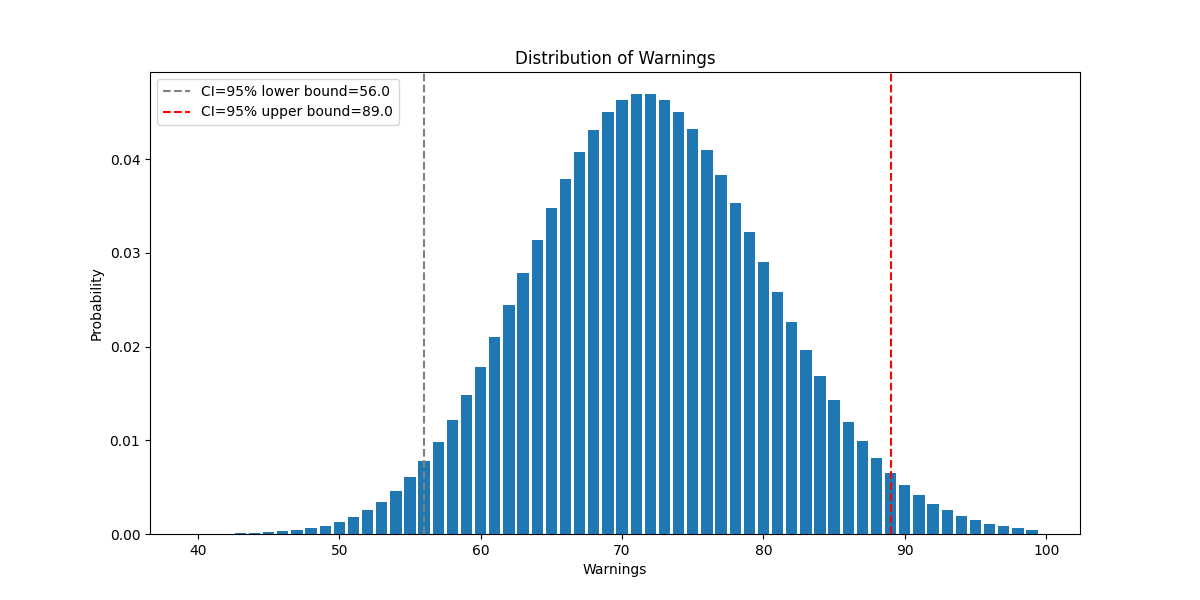
\includegraphics[scale=0.4]{example-report-gfx/eg_dist}
	\caption{报警次数的分布}
\end{figure}

\noindent
多图组合
\begin{figure}[h]
	\centering
	\begin{subfigure}{0.4\textwidth}
		\centering
		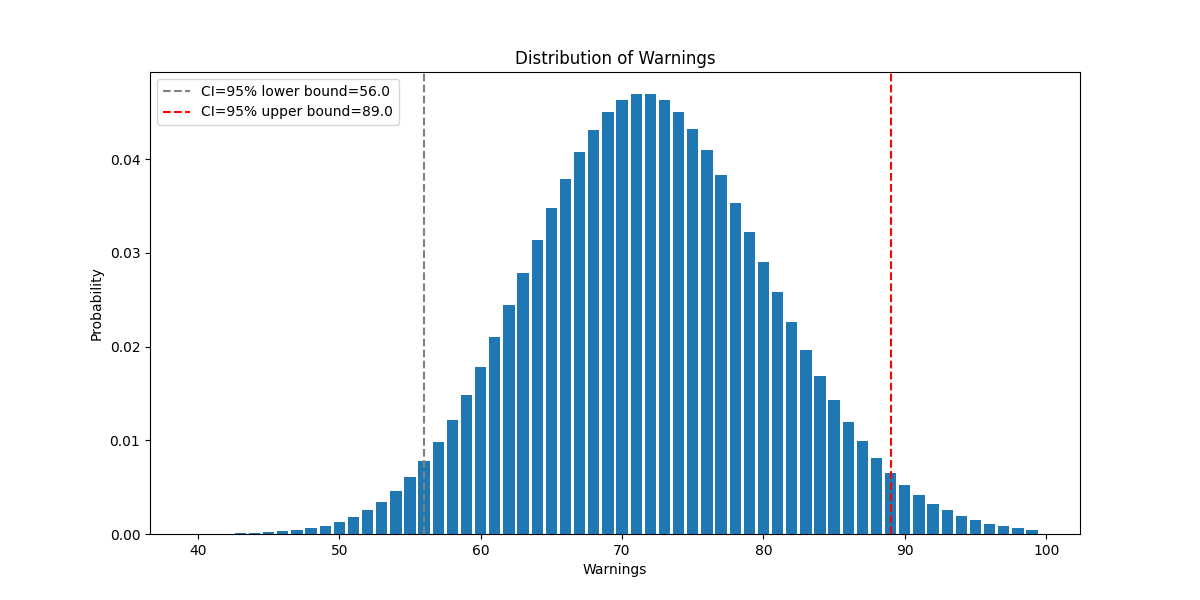
\includegraphics[width=\textwidth]{example-report-gfx/eg_dist}
		\caption{图1}
		\label{fig:image1}
	\end{subfigure}
	\quad 
	\begin{subfigure}{0.4\textwidth}
		\centering
		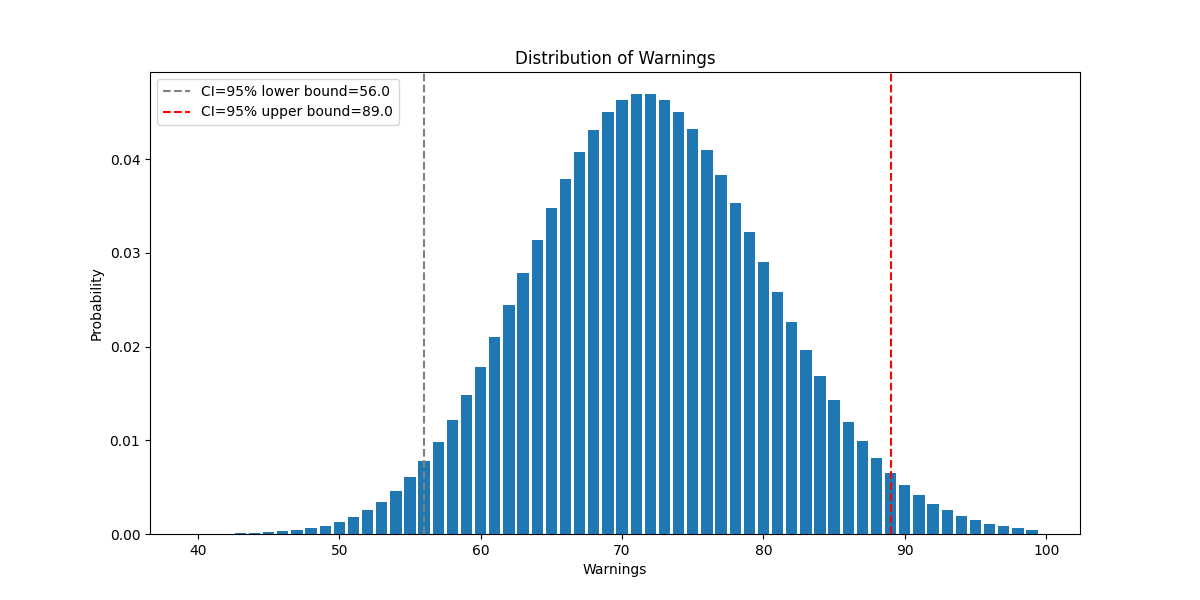
\includegraphics[width=\textwidth]{example-report-gfx/eg_dist}
		\caption{图2}
		\label{fig:image2}
	\end{subfigure}
	
	\vspace{6pt}
	
	\begin{subfigure}{0.4\textwidth}
		\centering
		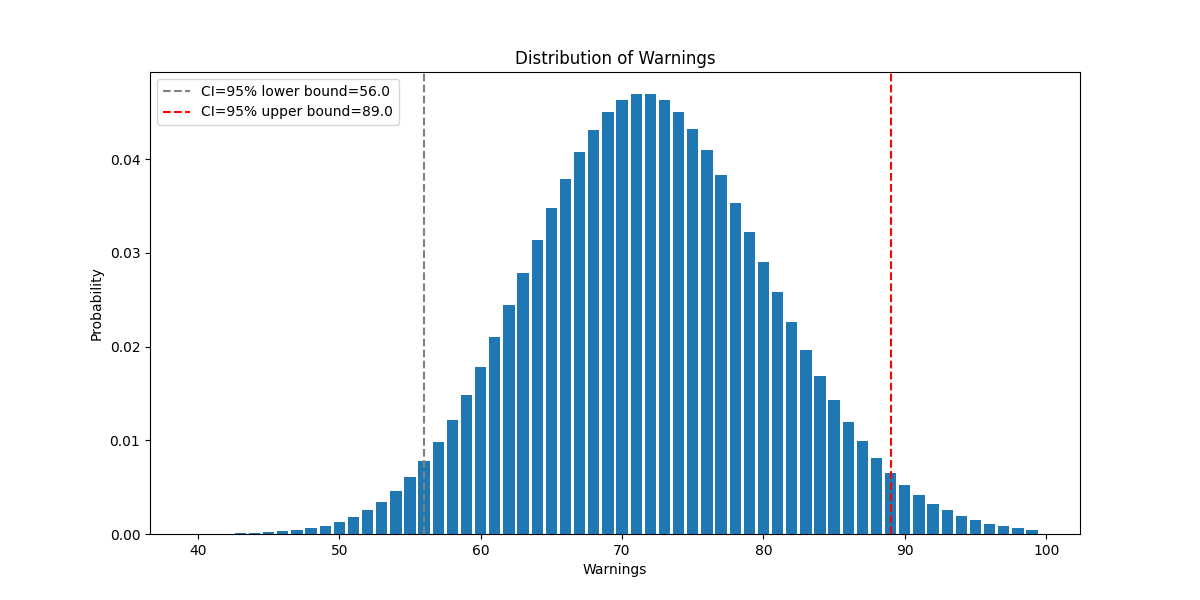
\includegraphics[width=\textwidth]{example-report-gfx/eg_dist}
		\caption{图3}
		\label{fig:image3}
	\end{subfigure}
	\quad
	\begin{subfigure}{0.4\textwidth}
		\centering
		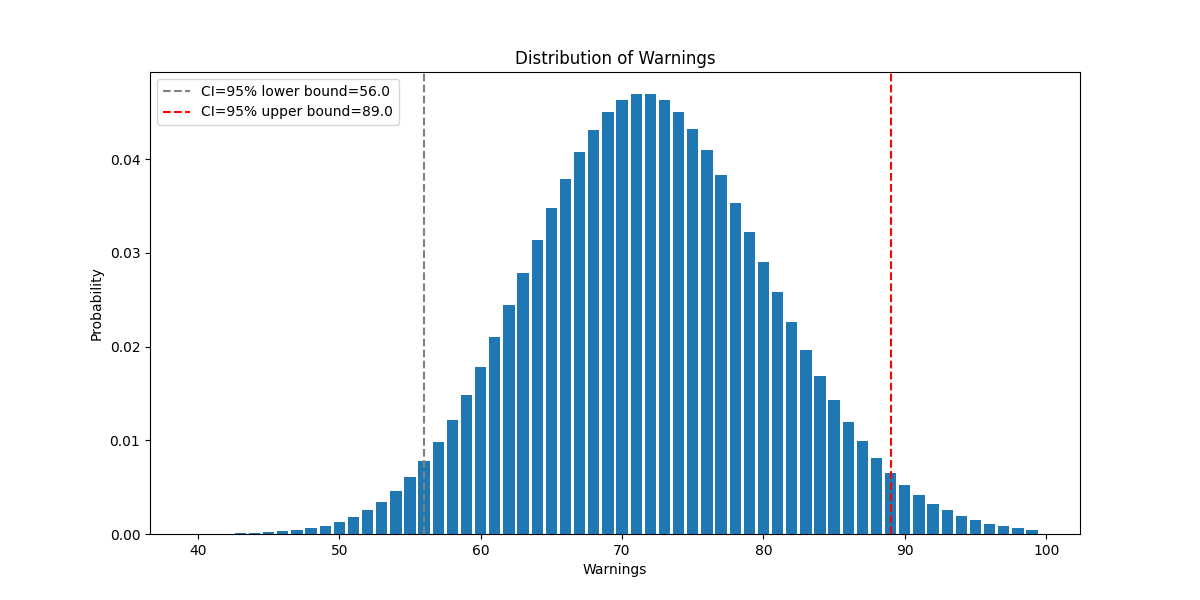
\includegraphics[width=\textwidth]{example-report-gfx/eg_dist}
		\caption{图4}
		\label{fig:image4}
	\end{subfigure}
	\caption{四张图}
\end{figure}

\noindent 旋转图片
\begin{center}
	\begin{tikzpicture}
		\node[rotate=30] at (0,0) {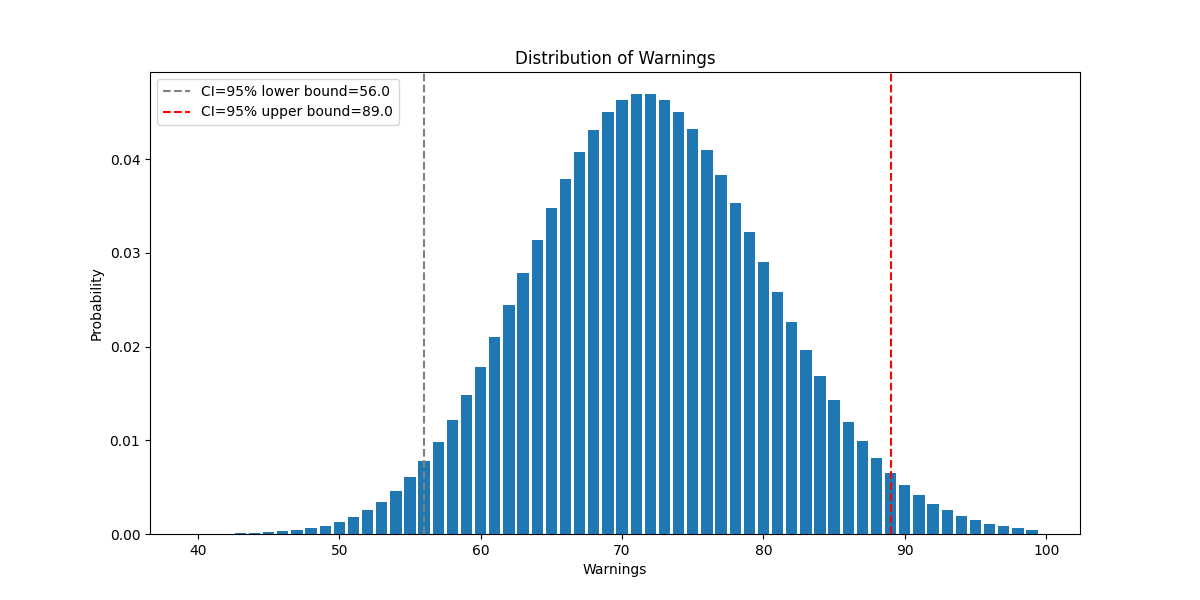
\includegraphics[width=120pt]{example-report-gfx/eg_dist}};
	\end{tikzpicture}
\end{center}
	
	
\section{Tikz 画图}

用 Tikz 画的流程图。

% Drawing part, node distance is 1.5 cm and every node
% is prefilled with white background
\begin{tikzpicture}[node distance=1.5cm,
	every node/.style={fill=white, font=\sffamily}, align=center]
	% Specification of nodes (position, etc.)
	
	\tikzset{%
		>={Latex[width=2mm,length=2mm]},
		% Specifications for style of nodes:
		base/.style = {rectangle, rounded corners, draw=black,
			minimum width=4cm, minimum height=1cm,
			text centered, font=\sffamily},
		activityStarts/.style = {base, fill=blue!30},
		startstop/.style = {base, fill=red!30},
		activityRuns/.style = {base, fill=green!30},
		process/.style = {base, minimum width=2.5cm, fill=orange!15,
			font=\ttfamily},
	}
	
	\node (start)             [activityStarts]              {Activity starts};
	\node (onCreateBlock)     [process, below of=start]          {onCreate()};
	\node (onStartBlock)      [process, below of=onCreateBlock]   {onStart()};
	\node (onResumeBlock)     [process, below of=onStartBlock]   {onResume()};
	\node (activityRuns)      [activityRuns, below of=onResumeBlock]
	{Activity is running};
	\node (onPauseBlock)      [process, below of=activityRuns, yshift=-1cm]
	{onPause()};
	\node (onStopBlock)       [process, below of=onPauseBlock, yshift=-1cm]
	{onStop()};
	\node (onDestroyBlock)    [process, below of=onStopBlock, yshift=-1cm] 
	{onDestroy()};
	\node (onRestartBlock)    [process, right of=onStartBlock, xshift=4cm]
	{onRestart()};
	\node (ActivityEnds)      [startstop, left of=activityRuns, xshift=-4cm]
	{Process is killed};
	\node (ActivityDestroyed) [startstop, below of=onDestroyBlock]
	{Activity is shut down};     
	% Specification of lines between nodes specified above
	% with aditional nodes for description 
	\draw[->]             (start) -- (onCreateBlock);
	\draw[->]     (onCreateBlock) -- (onStartBlock);
	\draw[->]      (onStartBlock) -- (onResumeBlock);
	\draw[->]     (onResumeBlock) -- (activityRuns);
	\draw[->]      (activityRuns) -- node[text width=4cm]
	{Another activity comes in
		front of the activity} (onPauseBlock);
	\draw[->]      (onPauseBlock) -- node {The activity is no longer visible}
	(onStopBlock);
	\draw[->]       (onStopBlock) -- node {The activity is shut down by
		user or system} (onDestroyBlock);
	\draw[->]    (onRestartBlock) -- (onStartBlock);
	\draw[->]       (onStopBlock) -| node[yshift=1.25cm, text width=3cm]
	{The activity comes to the foreground}
	(onRestartBlock);
	\draw[->]    (onDestroyBlock) -- (ActivityDestroyed);
	\draw[->]      (onPauseBlock) -| node(priorityXMemory)
	{higher priority $\rightarrow$ more memory}
	(ActivityEnds);
	\draw           (onStopBlock) -| (priorityXMemory);
	\draw[->]     (ActivityEnds)  |- node [yshift=-2cm, text width=3.1cm]
	{User navigates back to the activity}
	(onCreateBlock);
	\draw[->] (onPauseBlock.east) -- ++(2.6,0) -- ++(0,2) -- ++(0,2) --                
	node[xshift=1.2cm,yshift=-1.5cm, text width=2.5cm]
	{The activity comes to the foreground}(onResumeBlock.east);
\end{tikzpicture}


\section{字体样式}

\begin{itemize}
	\item \textbf{人爽事成}
	\item \uline{划重点}
	\item \uuline{重点是划两次} 
	\item \uwave{波浪线是不是直线?}
	\item \sout{删掉但是看得见} 
	\item \xout{这就看得有点费劲了} 
\end{itemize}

\section{代码}

\noindent 行内代码 \lstinline{$ cat /etc/shells} \\

\noindent 命令行
\begin{lstlisting}[language=Bash]
$ cat /etc/shells
\end{lstlisting}

\begin{lstlisting}
$ git pull [<options>] [<repository> [<refspec>…​]]
\end{lstlisting}

\vspace*{2ex}

\noindent 代码块

\begin{lstlisting}[language=Python, caption={Python 示例}]
def factorial(n):  
    # Returns the factorial of n. 
    if n == 0:
        return 1
    else:
        return n * factorial(n - 1)

if __name__ == '__main__':
    result = factorial(5)
    print("The result is ", result)
\end{lstlisting}


\begin{lstlisting}[language=Java, caption={Java 示例}]
public class HelloWorld {
    public static void main(String[] args) {
        System.out.println("Hello World");
    }
}
\end{lstlisting}

\begin{lstlisting}[caption={伪代码}, 
	emph={[1]procedure, if, return, else, end}, 
	emphstyle={[1]\color{blue}}, 
	emph={[2]quickSort}, 
	emphstyle={[2]\color{red}}]
procedure quickSort(left, right)
    if right-left <= 0
        return
    else     
        pivot = A[right]
        partition = partitionFunc(left, right, pivot)
        quickSort(left,partition-1)
        quickSort(partition+1,right)    
    end if		
end procedure
\end{lstlisting}

\section{文本框}

朴素的文本框
\begin{tcolorbox}[
	colback=white, 
	colframe=gray, 
	sharp corners, 
	leftrule={2pt}, rightrule={0.5pt}, toprule={0.5pt}, bottomrule={0.5pt}, 
	left={2pt}, right={2pt}, top={3pt}, bottom={3pt}
	]
	tcolorbox 宏包是 Thomas F. Sturm 开发的一个用于绘制彩色文本框的宏包 tcolorbox 底层基于 pgf,功能也是十分强大。
\end{tcolorbox}

\noindent 带标题和颜色的文本框

\begin{tcolorbox}[
	colback=white, 
	colframe=blue!15, 
	sharp corners, 
	coltitle=black, 
	left={2pt}, right={2pt}, top={3pt}, bottom={3pt}, 
	title = {注意事项}]
	This is a \textbf{tcolorbox} with title.
	\tcblower
	Here, you see the lower part of the box.
\end{tcolorbox}
	
\end{document}